% Drawing 74/02-4 -- folder 74, batch 02, archive page 23 (PDF page 24).
% Transcription: au bas de la page, quatre figures : un prisme aux sommets $c$, $b$, $t$, $t'$, $s$, $s'$, $a$, $a'$ ; un triangle dans lequel sont emboîtés deux angles de même sommet ; un double cône de sommets $s$ (en haut) et $s'$ (en bas), dont la ceinture porte $a$, $b'$, $c$, $a'$, $c'$, $b$, à côté d'un carré de $3 \times 3$ points ; un autre double cône analogue, de sommets $s'$ et $s$, portant $a$, $b'$, $c'$, $b$, $c$, $a'$ et des points $\alpha$, $\beta$, $\gamma$ à l'intérieur. Une croix au bas de la page.
% Kind: four figures (prism, nested angles, two double cones, 3x3 points). Method 2 (schematic redraw from the facsimile). Status: ok.
% Notes: Left to right, every stroke redrawn where it lies on the page. A prism: vertices a, a' (circled), s', t', s, t (circled), c, b and a circled a in the middle; strokes a-a'-s' (one stroke), a-t (level), a'-t' (interrupted by the labels a' and s, drawn as two pieces), s'-t' (curved), s'-s, s-t (curved), s down to the circled a, a-c, c-b, c to the circled a (bold), the circled a to b (curved), t-b (bold), t-t', and, thin, c towards a', b-t' and a short stroke down from s'. A triangle with two angles nested in it: the three points on its left joined to its upper and lower right corners. A 3x3 square of points. Below, two double cones: the first with apex s' at the top and s at the bottom, belt b', a, c', b, a', c, the curves s'-b' and s'-c', a thick stroke from s' down past c' that bends round to a', the inner curve from a down to a', the strokes from b' and from b towards the middle, the two short arrows inside, a stroke from c inwards, the points alpha, beta, gamma with their labels inside, and from c, from a point below it and from b down to s; the second with apex s at the top and s' (a blot) at the bottom, belt a, b', c, a', b, c' (no stroke a-a' on the page), s-a, s-c-a', b'-c, a-b', the thick axis from s down to the middle, a pencil stroke from s down to the right, the thin vertical below b', the doubled thick stroke above s', and c', b and a' joined to s'. Disagreement: the transcription gives alpha, beta, gamma to the second cone and puts the 3x3 square beside the first; on the page alpha, beta, gamma sit inside the first (left) cone and the square stands beside the second, above it (settled by a machine pass on the facsimile, 2026-11-12). Nothing is struck. The pairs (alpha, b'), ... at the right edge are text; the short vertical stroke left of the second cone, under the nested angles, is not part of a figure and is not drawn. Labels at \small, the figure drawn at 1.5 mm per unit so that they keep their places. Redrawn 2026-11-09 (issue 128); overlay check 2026-11-13 (issue 147) found the prism 2 to 3 units off and the inner edges a reading. Second pass 2026-11-14 (issue 147, Claude claude-opus-5-5): every stroke and label re-read on 30 to 40 px/unit gridded crops of the 400 dpi colour scan and redrawn there (s' of the second cone was 4 units too low, the nested angles and the square of points 1 to 2 units off, a stroke a-a' that the page does not have is removed). Rasterised by the session's previewer (not compiled: no TeX in the session) and laid over the crop: every stroke, point and label lies on its ink to within about 1 unit. Not checked by a reader.
% Coordinates: 1 unit = 1.5 mm = 1/100 of the crop width (bbox in page fractions: [0.08, 0.53, 0.78, 0.85]).
% Redrawn by Claude (claude-opus-5-5), issue #73, 2026-11-09; not checked by a human; not compiled (no TeX in the session).
% Checked by Claude (claude-opus-5-5) 2026-11-13 (issue #147): overlaid on the 300 dpi colour facsimile; not compiled (no TeX in the session). Status: partial.
% Second pass by Claude (claude-opus-5-5) 2026-11-14 (issue #147): redrawn stroke by stroke from the 400 dpi colour facsimile, overlaid on a grid; not compiled (no TeX in the session). Status: ok.
% Rights: reproduces part of the work -- behind RENDER_TRANSCRIPTS, never published by itself.
\documentclass[tikz,border=3pt]{standalone}
\usepackage{amsmath,amssymb}
\usetikzlibrary{patterns,arrows.meta}
\tikzset{pencil/.style={black!45}, struck/.style={black!35}, mark/.style={circle,draw,inner sep=1.3pt}, pt/.style={circle,fill,inner sep=0.9pt}, opt/.style={circle,draw,fill=white,inner sep=1.1pt}}
\begin{document}
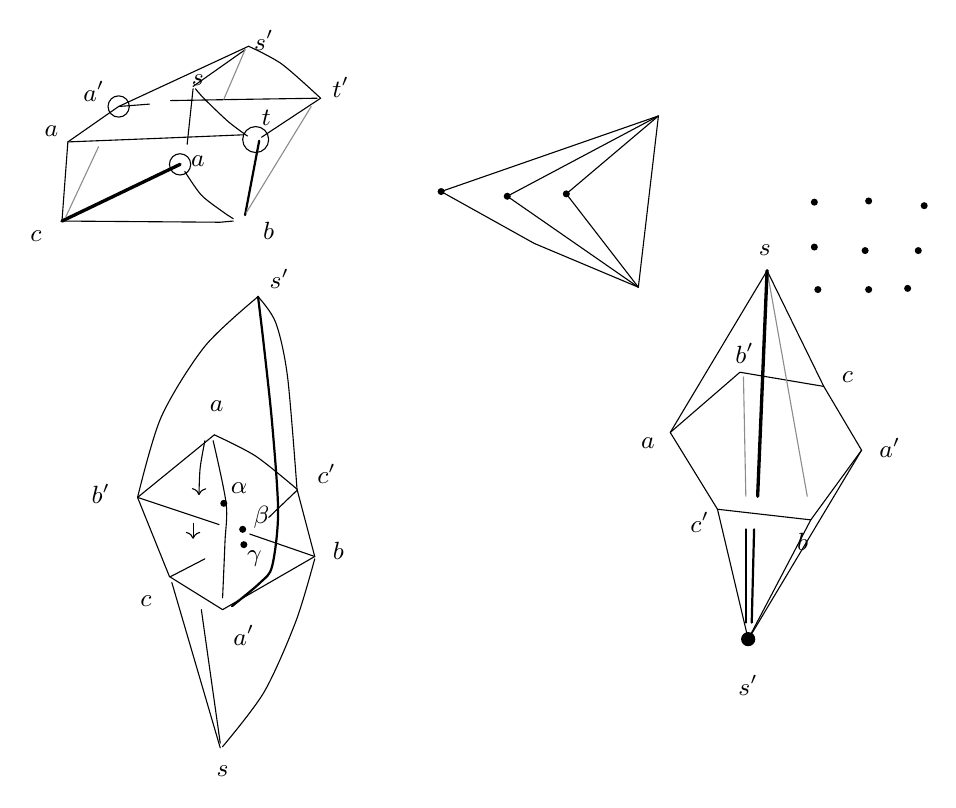
\begin{tikzpicture}[x=1.5mm,y=1.5mm,line cap=round,line join=round,font=\scriptsize]
\draw (17.4,-9.4) -- (21.7,-6.4) -- (32.7,-1.3);
\draw (17.4,-9.4) -- (25,-9.1) -- (32.2,-8.8);
\draw (21.7,-6.4) -- (24.3,-6.2);
\draw (26.1,-5.9) -- (32,-5.8) -- (38.5,-5.7);
\draw plot[smooth] coordinates {(32.7,-1.3) (35.5,-2.8) (38.8,-5.7)};
\draw (32.4,-1.6) -- (28.0,-4.7);
\draw[pencil] (32.4,-1.6) -- (30.6,-5.8);
\draw plot[smooth] coordinates {(28.2,-4.9) (29,-5.8) (31,-7.7) (32.6,-8.9)};
\draw (28.0,-4.9) -- (27.5,-9.6);
\draw (17.4,-9.4) -- (16.9,-16.1);
\draw[very thick] (16.9,-16.1) -- (26.9,-11.3);
\draw (16.9,-16.1) -- (30.3,-16.2) -- (31.4,-16.1);
\draw[pencil] (17.2,-15.8) -- (20,-9.8);
\draw plot[smooth] coordinates {(27.3,-11.9) (28.7,-13.9) (30.5,-15.3) (31.4,-15.9)};
\draw[thick] (33.6,-9.3) -- (32.4,-15.6);
\draw[pencil] (32.5,-15.4) -- (38,-6.4);
\draw (33.8,-9.0) -- (38.8,-5.7);
\draw (21.7,-6.4) circle[radius=0.9];
\draw (33.3,-9.2) circle[radius=1.1];
\draw (26.9,-11.3) circle[radius=0.9];
\node[inner sep=1pt] at (16.0,-8.5) {\small $a$};
\node[inner sep=1pt] at (19.6,-5.1) {\small $a'$};
\node[inner sep=1pt] at (34.0,-0.8) {\small $s'$};
\node[inner sep=1pt] at (40.5,-4.8) {\small $t'$};
\node[inner sep=1pt] at (28.4,-4.2) {\small $s$};
\node[inner sep=1pt] at (34.2,-7.4) {\small $t$};
\node[inner sep=1pt] at (28.4,-11.0) {\small $a$};
\node[inner sep=1pt] at (14.7,-17.4) {\small $c$};
\node[inner sep=1pt] at (34.4,-16.9) {\small $b$};
\draw (67.4,-7.2) -- (49,-13.6) -- (56.9,-18) -- (65.7,-21.7) -- cycle;
\draw (54.6,-14) -- (67.4,-7.2);
\draw (54.6,-14) -- (65.7,-21.7);
\draw (59.6,-13.8) -- (67.4,-7.2);
\draw (59.6,-13.8) -- (65.7,-21.7);
\node[pt] at (49,-13.6) {};
\node[pt] at (54.6,-14) {};
\node[pt] at (59.6,-13.8) {};
\node[pt] at (80.6,-14.5) {};
\node[pt] at (85.2,-14.4) {};
\node[pt] at (89.9,-14.8) {};
\node[pt] at (80.6,-18.3) {};
\node[pt] at (84.9,-18.6) {};
\node[pt] at (89.4,-18.6) {};
\node[pt] at (80.9,-21.9) {};
\node[pt] at (85.2,-21.9) {};
\node[pt] at (88.5,-21.8) {};
\draw plot[smooth] coordinates {(33.5,-22.5) (29,-26.7) (25.3,-32.7) (23.3,-39.5)};
\draw plot[smooth] coordinates {(33.5,-22.5) (35,-24.7) (36,-29.3) (36.8,-38.8)};
\draw[thick] plot[smooth] coordinates {(33.5,-22.5) (34,-26.7) (34.7,-33.3) (35.2,-40.7) (34.7,-45.3) (33.7,-46.7) (31.3,-48.7)};
\draw (29.8,-34.2) -- (23.3,-39.5);
\draw plot[smooth] coordinates {(29.8,-34.2) (33.3,-36) (36.8,-38.8)};
\draw (23.3,-39.5) -- (30.2,-41.8);
\draw (23.3,-39.5) -- (26,-46.2) -- (30.5,-49) -- (38.3,-44.5) -- (36.8,-38.8);
\draw (38.3,-44.5) -- (32.8,-42.6);
\draw (36.8,-38.9) -- (34.4,-41.2);
\draw plot[smooth] coordinates {(29.7,-34.7) (30.8,-40) (30.7,-43.3) (30.5,-48)};
\draw[->] plot[smooth] coordinates {(29,-34.7) (28.6,-37) (28.5,-39.3)};
\draw[->] (28,-41.7) -- (28,-43);
\draw (26.1,-46.2) -- (29,-44.7);
\draw (26.2,-46.7) -- (30.3,-60.7);
\draw (28.7,-49) -- (30.3,-60.3);
\draw plot[smooth] coordinates {(38.3,-44.7) (36.7,-50) (34,-56) (30.5,-60.6)};
\node[pt] at (30.6,-40) {};
\node[pt] at (32.2,-42.2) {};
\node[pt] at (32.3,-43.5) {};
\node[inner sep=1pt] at (31.9,-38.7) {\small $\alpha$};
\node[inner sep=1pt] at (33.8,-41.2) {\small $\beta$};
\node[inner sep=1pt] at (33.2,-44.7) {\small $\gamma$};
\node[inner sep=1pt] at (35.3,-21) {\small $s'$};
\node[inner sep=1pt] at (30.5,-62.7) {\small $s$};
\node[inner sep=1pt] at (20.2,-39.2) {\small $b'$};
\node[inner sep=1pt] at (30,-31.8) {\small $a$};
\node[inner sep=1pt] at (39.3,-37.5) {\small $c'$};
\node[inner sep=1pt] at (40.3,-44) {\small $b$};
\node[inner sep=1pt] at (32.3,-51.2) {\small $a'$};
\node[inner sep=1pt] at (24,-48.3) {\small $c$};
\draw (76.6,-20.3) -- (68.4,-34) -- (72.4,-40.5) -- (80.3,-41.4) -- (84.6,-35.5) -- (81.4,-30.1) -- cycle;
\draw (68.4,-34) -- (74.3,-28.9) -- (81.4,-30.1);
\draw[pencil] (74.6,-29.3) -- (74.8,-39.4);
\draw[pencil] (76.6,-20.3) -- (80,-39.4);
\draw[very thick] (76.6,-20.3) -- (75.8,-39.4);
\draw (72.4,-40.5) -- (75,-51.5);
\draw (80.3,-41.4) -- (75,-51.5);
\draw (84.6,-35.5) -- (75.2,-51.2);
\draw[thick] (74.8,-42.2) -- (74.8,-50.1);
\draw[thick] (75.5,-42.2) -- (75.3,-50.1);
\fill (75,-51.5) circle[radius=0.6];
\node[inner sep=1pt] at (76.4,-18.6) {\small $s$};
\node[inner sep=1pt] at (75,-55.4) {\small $s'$};
\node[inner sep=1pt] at (66.5,-34.9) {\small $a$};
\node[inner sep=1pt] at (74.7,-27.3) {\small $b'$};
\node[inner sep=1pt] at (83.4,-29.3) {\small $c$};
\node[inner sep=1pt] at (87,-35.3) {\small $a'$};
\node[inner sep=1pt] at (79.6,-43.3) {\small $b$};
\node[inner sep=1pt] at (70.9,-41.6) {\small $c'$};
\end{tikzpicture}
\end{document}
